% Sankalp - Rural Education Management System Presentation
% Compile with: pdflatex presentation.tex
% Place images in an 'images' folder in the same directory

\documentclass[aspectratio=169]{beamer}
\usetheme{Madrid}
\usecolortheme{default}

% Packages
\usepackage{graphicx}
\usepackage{tikz}

% Color definitions
\definecolor{primarycolor}{RGB}{26, 23, 20}
\definecolor{accentcolor}{RGB}{194, 120, 3}
\definecolor{successcolor}{RGB}{34, 197, 94}

% Title page information
\title{\textbf{Sankalp}}
\subtitle{Rural Education Management System}
\author{Project Team}
\date{\today}

\begin{document}

% Title slide
\begin{frame}
    \titlepage
\end{frame}

% Table of contents
\begin{frame}{Outline}
    \tableofcontents
\end{frame}

%=============================================================================
% SECTION 1: THE PROBLEM
%=============================================================================
\section{The Problem}

\begin{frame}{Rural Education Challenges}
    \begin{columns}
        \column{0.6\textwidth}
        \textbf{Current Situation:}
        \begin{itemize}
            \item 6+ rural villages
            \item 47+ students
            \item Weekend volunteer programs
            \item Manual paper-based tracking
        \end{itemize}
        
        \vspace{1em}
        
        \textbf{Key Challenges:}
        \begin{itemize}
            \item No centralized system
            \item Difficult to track impact
            \item Time-consuming admin work
        \end{itemize}
        
        \column{0.4\textwidth}
        \centering
        % Add your village/classroom image here
        \fbox{\parbox{0.9\textwidth}{
            \centering
            \vspace{2cm}
            \textit{[Village Image]}
            \vspace{2cm}
        }}
    \end{columns}
\end{frame}

%=============================================================================
% SECTION 2: OUR SOLUTION
%=============================================================================
\section{Our Solution}

\begin{frame}{Sankalp Platform}
    \begin{center}
        \Large\textbf{A Digital Platform for}\\
        \Large\textbf{Volunteer-Driven Rural Education}
    \end{center}
    
    \vspace{2em}
    
    \begin{columns}
        \column{0.33\textwidth}
        \centering
        \textbf{Volunteer\\Management}\\
        \small Check-in, session logging
        
        \column{0.33\textwidth}
        \centering
        \textbf{Analytics\\Dashboard}\\
        \small Real-time insights
        
        \column{0.33\textwidth}
        \centering
        \textbf{Student\\Tracking}\\
        \small Progress monitoring
    \end{columns}
\end{frame}

\begin{frame}{Key Features}
    \begin{columns}
        \column{0.5\textwidth}
        \textbf{For Administrators:}
        \begin{itemize}
            \item Event management
            \item Volunteer analytics
            \item Student database
            \item Progress reports
        \end{itemize}
        
        \vspace{1em}
        
        \textbf{For Volunteers:}
        \begin{itemize}
            \item Quick check-in
            \item Session logging
            \item Attendance history
        \end{itemize}
        
        \column{0.5\textwidth}
        \centering
        % Add dashboard screenshot here
        \fbox{\parbox{0.9\textwidth}{
            \centering
            \vspace{3cm}
            \textit{[Dashboard Screenshot]}
            \vspace{3cm}
        }}
    \end{columns}
\end{frame}

\begin{frame}{User Experience}
    \begin{columns}
        \column{0.5\textwidth}
        \centering
        % Add login page screenshot
        \fbox{\parbox{0.9\textwidth}{
            \centering
            \vspace{2.5cm}
            \textit{[Login Page]}
            \vspace{2.5cm}
        }}
        
        \column{0.5\textwidth}
        \textbf{Smart Features:}
        \begin{itemize}
            \item Role detection from email
            \item Mobile-first design
            \item Touch-optimized
            \item No zoom on mobile
        \end{itemize}
        
        \vspace{1em}
        
        \textbf{Accessibility:}
        \begin{itemize}
            \item High contrast
            \item Keyboard navigation
            \item Screen reader support
        \end{itemize}
    \end{columns}
\end{frame}

%=============================================================================
% SECTION 3: TECHNICAL OVERVIEW
%=============================================================================
\section{Technical Overview}

\begin{frame}{Technology Stack}
    \begin{center}
        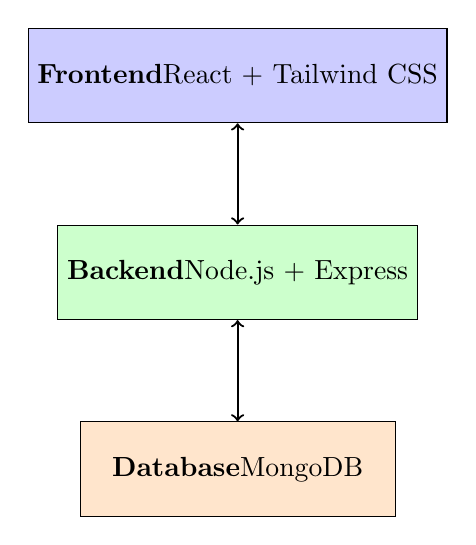
\begin{tikzpicture}[node distance=2.5cm]
            \node[draw, rectangle, minimum width=4cm, minimum height=1.2cm, fill=blue!20] (frontend) {\textbf{Frontend}\\React + Tailwind CSS};
            \node[draw, rectangle, minimum width=4cm, minimum height=1.2cm, fill=green!20, below of=frontend] (backend) {\textbf{Backend}\\Node.js + Express};
            \node[draw, rectangle, minimum width=4cm, minimum height=1.2cm, fill=orange!20, below of=backend] (database) {\textbf{Database}\\MongoDB};
            
            \draw[<->, thick] (frontend) -- (backend);
            \draw[<->, thick] (backend) -- (database);
        \end{tikzpicture}
    \end{center}
    
    \vspace{1em}
    
    \textbf{Modern MERN Stack:} MongoDB, Express.js, React, Node.js
\end{frame}

\begin{frame}{System Architecture}
    \begin{columns}
        \column{0.5\textwidth}
        \textbf{Frontend:}
        \begin{itemize}
            \item React.js
            \item Tailwind CSS
            \item Recharts
            \item Responsive design
        \end{itemize}
        
        \vspace{1em}
        
        \textbf{Backend:}
        \begin{itemize}
            \item Express.js API
            \item JWT authentication
            \item MongoDB database
        \end{itemize}
        
        \column{0.5\textwidth}
        \centering
        % Add architecture diagram or system flow
        \fbox{\parbox{0.9\textwidth}{
            \centering
            \vspace{3cm}
            \textit{[Architecture Diagram]}
            \vspace{3cm}
        }}
    \end{columns}
\end{frame}

\begin{frame}{Security Features}
    \begin{itemize}
        \item \textbf{Authentication:} JWT tokens, password hashing
        \item \textbf{Authorization:} Role-based access control
        \item \textbf{Validation:} Input sanitization, time-bound codes
        \item \textbf{Location:} Geofencing (1km radius)
    \end{itemize}
    
    \vspace{2em}
    
    \begin{center}
        % Add security flow diagram or screenshot
        \fbox{\parbox{0.6\textwidth}{
            \centering
            \vspace{2cm}
            \textit{[Security Flow]}
            \vspace{2cm}
        }}
    \end{center}
\end{frame}

%=============================================================================
% SECTION 4: IMPACT & RESULTS
%=============================================================================
\section{Impact \& Results}

\begin{frame}{Measurable Impact}
    \begin{columns}
        \column{0.5\textwidth}
        \textbf{Efficiency Gains:}
        \begin{itemize}
            \item 90\% less admin time
            \item Real-time tracking
            \item Instant reports
            \item Zero paper waste
        \end{itemize}
        
        \vspace{1em}
        
        \textbf{Current Scale:}
        \begin{itemize}
            \item 47+ students
            \item 6 villages
            \item 20+ volunteers
            \item 23+ sessions/month
        \end{itemize}
        
        \column{0.5\textwidth}
        \centering
        % Add analytics/charts screenshot
        \fbox{\parbox{0.9\textwidth}{
            \centering
            \vspace{3cm}
            \textit{[Analytics Dashboard]}
            \vspace{3cm}
        }}
    \end{columns}
\end{frame}

\begin{frame}{Student Progress Tracking}
    \begin{center}
        % Add student progress screenshot or village photos
        \fbox{\parbox{0.7\textwidth}{
            \centering
            \vspace{4cm}
            \textit{[Student Progress / Village Photos]}
            \vspace{4cm}
        }}
    \end{center}
    
    \vspace{1em}
    
    \textbf{Track:} Attendance, subjects taught, topics covered, performance
\end{frame}

\begin{frame}{Volunteer Engagement}
    \begin{columns}
        \column{0.5\textwidth}
        \centering
        % Add volunteer rankings screenshot
        \fbox{\parbox{0.9\textwidth}{
            \centering
            \vspace{2.5cm}
            \textit{[Volunteer Rankings]}
            \vspace{2.5cm}
        }}
        
        \column{0.5\textwidth}
        \textbf{Features:}
        \begin{itemize}
            \item Participation rankings
            \item Attendance history
            \item Session logs
            \item Performance metrics
        \end{itemize}
        
        \vspace{1em}
        
        \textbf{Benefits:}
        \begin{itemize}
            \item Motivates volunteers
            \item Recognizes contributions
            \item Tracks commitment
        \end{itemize}
    \end{columns}
\end{frame}

%=============================================================================
% SECTION 5: FUTURE VISION
%=============================================================================
\section{Future Vision}

\begin{frame}{Roadmap}
    \textbf{Short Term:}
    \begin{itemize}
        \item SMS notifications
        \item Offline mode
        \item Multi-language support
    \end{itemize}
    
    \vspace{0.5em}
    
    \textbf{Medium Term:}
    \begin{itemize}
        \item AI teaching recommendations
        \item Video recording
        \item Parent portal
    \end{itemize}
    
    \vspace{0.5em}
    
    \textbf{Long Term:}
    \begin{itemize}
        \item Mobile app
        \item Multi-organization support
        \item Government integration
    \end{itemize}
\end{frame}

\begin{frame}{Scalability}
    \begin{center}
        \Large\textbf{Built to Scale}
    \end{center}
    
    \vspace{2em}
    
    \begin{columns}
        \column{0.5\textwidth}
        \textbf{Technical:}
        \begin{itemize}
            \item Cloud deployment
            \item Load balancing
            \item Database sharding
        \end{itemize}
        
        \column{0.5\textwidth}
        \textbf{Organizational:}
        \begin{itemize}
            \item Multi-tenant
            \item Custom branding
            \item API integration
        \end{itemize}
    \end{columns}
\end{frame}

%=============================================================================
% SECTION 6: CONCLUSION
%=============================================================================
\section{Conclusion}

\begin{frame}{Key Takeaways}
    \begin{enumerate}
        \item \textbf{Problem:} Manual, unstructured rural education tracking
        
        \vspace{0.5em}
        
        \item \textbf{Solution:} Digital platform for volunteer coordination
        
        \vspace{0.5em}
        
        \item \textbf{Technology:} Modern MERN stack, secure \& scalable
        
        \vspace{0.5em}
        
        \item \textbf{Impact:} 90\% efficiency gain, 47+ students benefiting
        
        \vspace{0.5em}
        
        \item \textbf{Future:} Ready to scale to multiple organizations
    \end{enumerate}
\end{frame}

\begin{frame}{Project Impact}
    \begin{center}
        % Add collage of village/student/volunteer photos
        \fbox{\parbox{0.8\textwidth}{
            \centering
            \vspace{4cm}
            \textit{[Project Photos Collage]}
            \vspace{4cm}
        }}
    \end{center}
    
    \vspace{1em}
    
    \begin{center}
        \textit{"Empowering rural communities through structured education"}
    \end{center}
\end{frame}

\begin{frame}
    \begin{center}
        \Huge\textbf{Thank You!}
        
        \vspace{2em}
        
        \Large Questions?
        
        \vspace{2em}
        
        \normalsize
        \textbf{GitHub:} github.com/kushagragarg15/sankalp-village-project
        
        \vspace{1em}
        
        \textit{"Education is the most powerful weapon\\which you can use to change the world."}\\
        \textit{— Nelson Mandela}
    \end{center}
\end{frame}

%=============================================================================
% APPENDIX - DEMO SLIDES
%=============================================================================
\appendix
\section{Demo Screenshots}

\begin{frame}{Login Page}
    \begin{center}
        % Full-screen login page screenshot
        \fbox{\parbox{0.9\textwidth}{
            \centering
            \vspace{5cm}
            \textit{[Login Page Screenshot]}\\
            \small Progressive role disclosure feature
            \vspace{5cm}
        }}
    \end{center}
\end{frame}

\begin{frame}{Dashboard}
    \begin{center}
        % Full-screen dashboard screenshot
        \fbox{\parbox{0.9\textwidth}{
            \centering
            \vspace{5cm}
            \textit{[Dashboard Screenshot]}\\
            \small Real-time metrics and quick actions
            \vspace{5cm}
        }}
    \end{center}
\end{frame}

\begin{frame}{Volunteer Sessions}
    \begin{center}
        % Full-screen volunteer sessions screenshot
        \fbox{\parbox{0.9\textwidth}{
            \centering
            \vspace{5cm}
            \textit{[Volunteer Sessions Screenshot]}\\
            \small Session registration and attendance
            \vspace{5cm}
        }}
    \end{center}
\end{frame}

\begin{frame}{Student Management}
    \begin{center}
        % Full-screen student list screenshot
        \fbox{\parbox{0.9\textwidth}{
            \centering
            \vspace{5cm}
            \textit{[Student Management Screenshot]}\\
            \small Student database and progress tracking
            \vspace{5cm}
        }}
    \end{center}
\end{frame}

\begin{frame}{Analytics}
    \begin{center}
        % Full-screen analytics screenshot
        \fbox{\parbox{0.9\textwidth}{
            \centering
            \vspace{5cm}
            \textit{[Analytics Screenshot]}\\
            \small Volunteer rankings and attendance reports
            \vspace{5cm}
        }}
    \end{center}
\end{frame}

\begin{frame}{Mobile View}
    \begin{center}
        % Mobile screenshots side by side
        \begin{columns}
            \column{0.33\textwidth}
            \centering
            \fbox{\parbox{0.9\textwidth}{
                \centering
                \vspace{3cm}
                \textit{[Mobile 1]}
                \vspace{3cm}
            }}
            
            \column{0.33\textwidth}
            \centering
            \fbox{\parbox{0.9\textwidth}{
                \centering
                \vspace{3cm}
                \textit{[Mobile 2]}
                \vspace{3cm}
            }}
            
            \column{0.33\textwidth}
            \centering
            \fbox{\parbox{0.9\textwidth}{
                \centering
                \vspace{3cm}
                \textit{[Mobile 3]}
                \vspace{3cm}
            }}
        \end{columns}
        
        \vspace{1em}
        \small Responsive design for all devices
    \end{center}
\end{frame}

\end{document}
